
\documentclass{llncs}
%
% additional packages added to comply wth format recommendations
%
\usepackage{makeidx}  % allows for indexgeneration
\usepackage[strings]{underscore} % allows underscore
\usepackage{float} % position tables inline
\usepackage{placeins}
\usepackage{caption}
\captionsetup[table]{singlelinecheck=false,
					labelfont=bf,
					justification=raggedright,
					labelsep=period}
\usepackage{textcomp}
\usepackage{colortbl}
\usepackage{graphicx}

\usepackage{subcaption}		% enables side-by-side figures
\captionsetup{compatibility = false}	% needed for subcaption package


% ... -=-=-=-=-=-=-=-=-=-=-=-=-=-=-=-=-=-=-=-=-=-=-=-=-=-=-=-=-=-=-=-=-=-=-=-=-
% ...	 directory paths for images
% ... -=-=-=-=-=-=-=-=-=-=-=-=-=-=-=-=-=-=-=-=-=-=-=-=-=-=-=-=-=-=-=-=-=-=-=-=-

\graphicspath{
    {.} % document root dir
    {images/}
}

\begin{document}

Figure ~\ref{figure : dataFeatureDevelopment}. \newline
\begin{figure}
  \begin{subfigure}[b]{0.5\textwidth}
    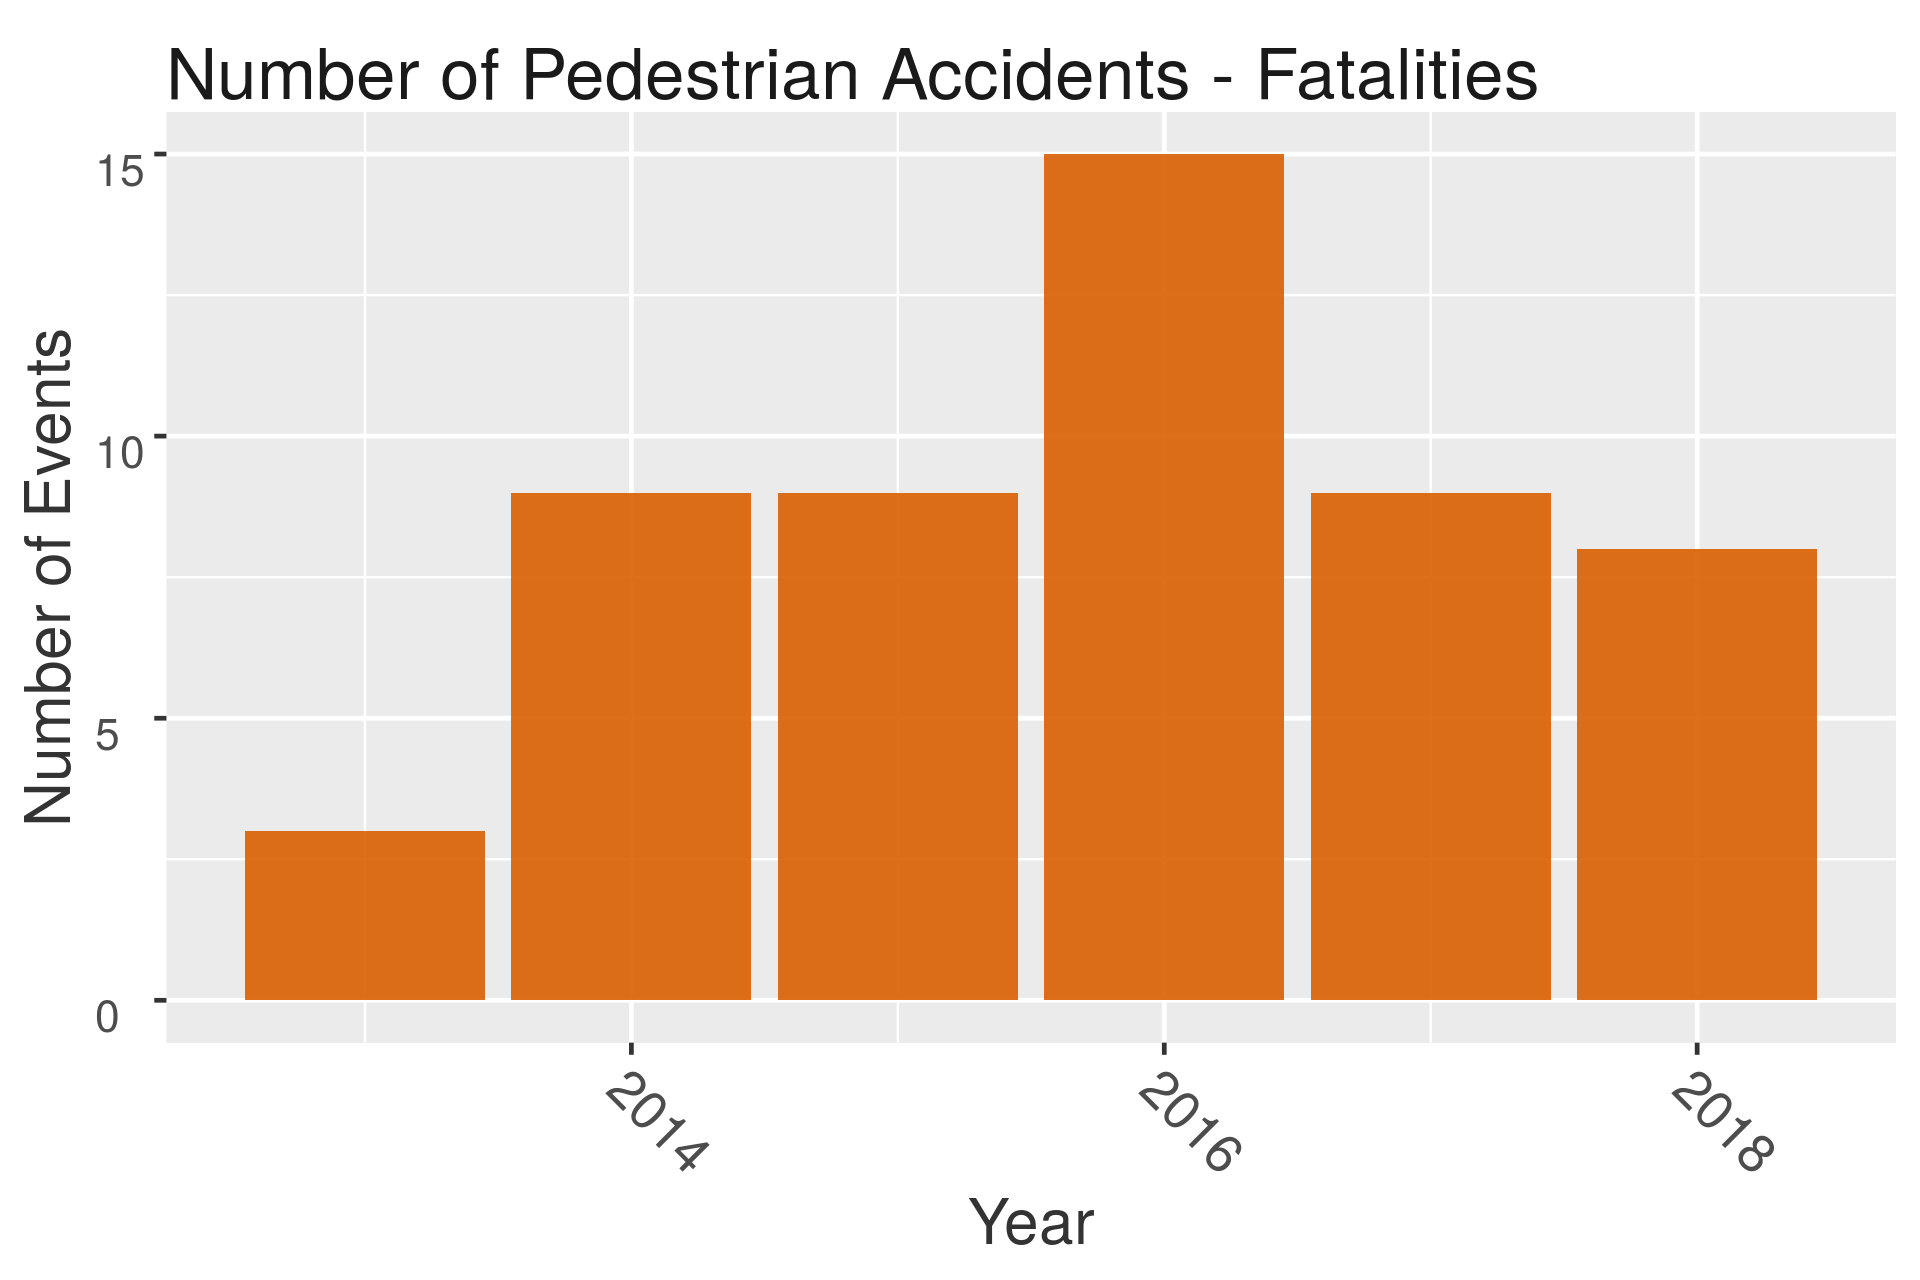
\includegraphics[width = \textwidth, height = \textheight, keepaspectratio]{pedestrianAccidentNumFatalities.png}
    \caption{Walk Score - Max values}
    \label{fig:1}
  \end{subfigure}
  %
  \begin{subfigure}[b]{0.5\textwidth}
    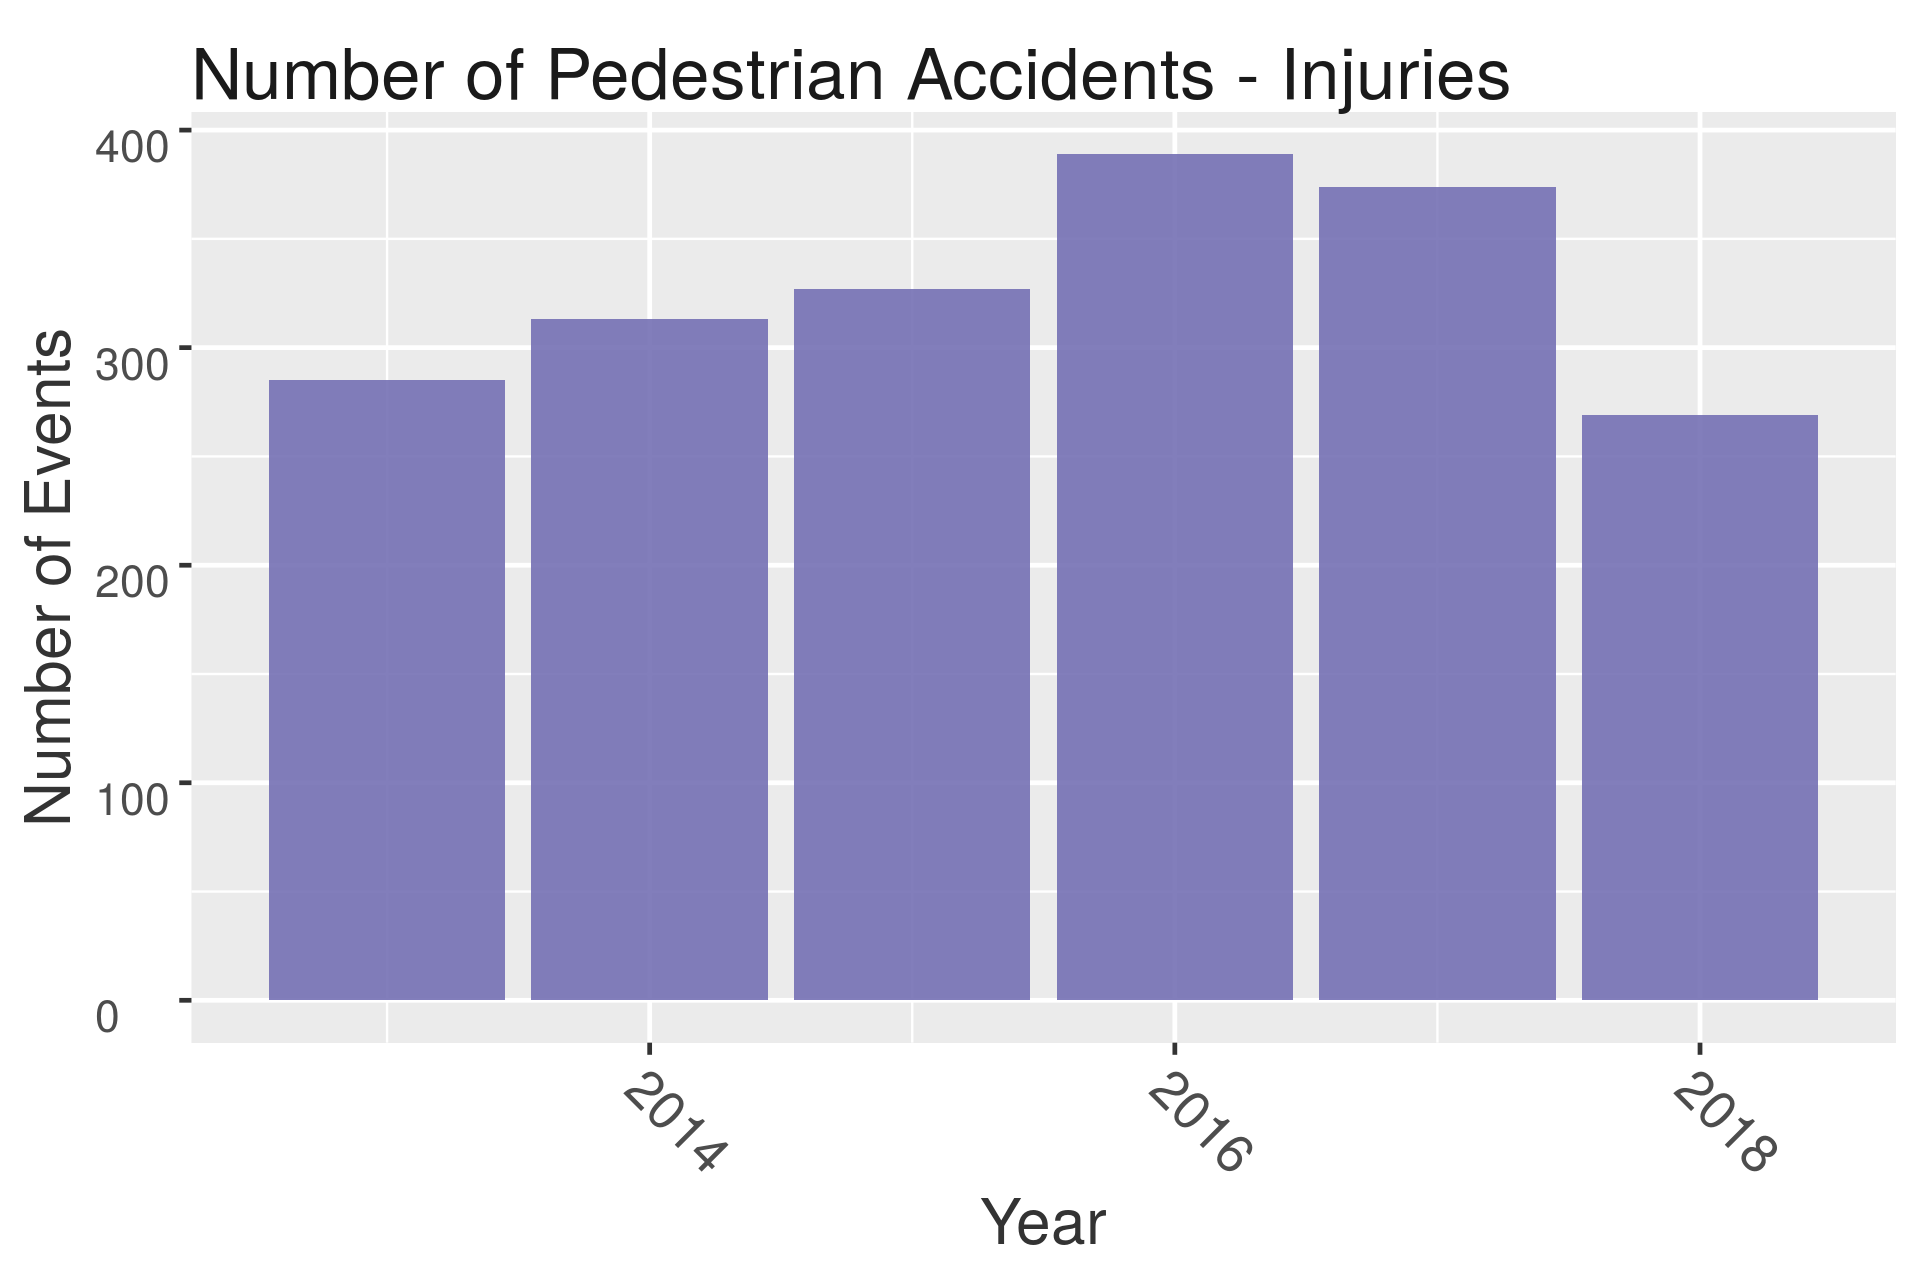
\includegraphics[width = \textwidth, height = \textheight, keepaspectratio]{pedestrianAccidentNumInjuries.png}
    \caption{Public Transportaton accessibility}
    \label{fig:2}
  \end{subfigure}
\end{figure}


\end{document}